\part{Foundation}

尽管 ECMAScript 是一个重要的标准,但它并不是 JavaScript 唯一的部分,当然,也不是唯一被标准化的部分。实际上,一个完整的 JavaScript 实现是由以下 3 个不同部分组成的:

\begin{compactitem}
\item 核心(ECMAScript)描述了该语言的语法和基本对象。
\item 文档对象模型(DOM),描述处理网页内容的方法和接口
\item 浏览器对象模型(BOM),描述与浏览器进行交互的方法和接口
\end{compactitem}


\vspace{-10pt}

\begin{figure}[!h]
\centering
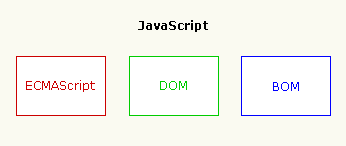
\includegraphics[scale=0.5]{js_arch.png}
\vspace{-20pt}
\caption{JavaScript模型}
\label{js_arch}
\end{figure}


在 ECMA-262 中,ECMAScript 符合性(conformance)有明确的定义。一个脚本语言必须满足以下四项基本原则:

\begin{compactitem}
\item 符合的实现必须按照 ECMA-262 中所描述的支持所有的“类型、值、对象、属性、函数和程序语言及语义”(ECMA-262,第一页)
\item 符合的实现必须支持 Unicode 字符标准(UCS)
\item 符合的实现可以增加没有在 ECMA-262 中指定的“额外类型、值、对象、属性和函数”。ECMA-262 将这些增加描述为规范中未给定的新对象或对象的新属性
\item 符合的实现可以支持没有在 ECMA-262 中定义的“程序和正则表达式语法”(意思是可以替换或者扩展内建的正则表达式支持)
\end{compactitem}

所有 ECMAScript 实现必须符合以上标准。

ECMAScript 仅仅是一个描述,定义了脚本语言的所有属性、方法和对象。其他语言可以实现 ECMAScript 来作为功能的基准,例如,JavaScript 就是这样:

\begin{figure}[!h]
\centering
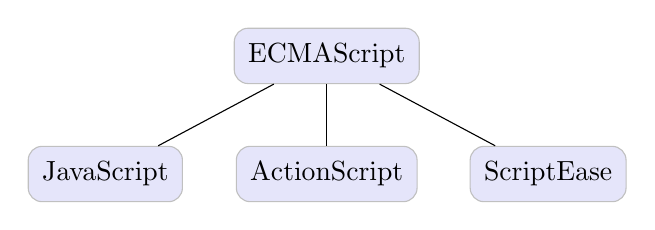
\begin{tikzpicture}[sibling distance=80pt]
\tikzset{
box/.style={ rectangle , rounded corners=5pt ,
minimum width=50pt , minimum height=20pt , inner sep=5pt ,
draw=Silver ,fill=Lavender }
}

\node[box]{ECMAScript}
	child {node[box] {JavaScript}}
	child {node[box] {ActionScript}}
	child {node[box] {ScriptEase}};

\end{tikzpicture}
\caption{ECMAScript实现}
\label{ECMAScript_implement}
\end{figure}

每个浏览器都有它自己的 ECMAScript 接口的实现,然后这个实现又被扩展,包含了 DOM 和 BOM。当然还有其他实现并扩展了 ECMAScript 的语言,例如 Windows 脚本宿主(Windows Scripting Host, WSH)、Macromedia 在 Flash 和 Director MX 中的 ActionScript,以及 Nombas ScriptEase。

ECMAScript 并不与任何具体浏览器相绑定,实际上,它也没有提到用于任何用户输入输出的方法(这点与 C 这类语言不同,它需要依赖外部的库来完成这类任务)。

ECMA-262 标准(第 2 段)中对ECMAScript的描述如下:

\vspace{20pt}

\textcolor{Blue}{“ECMAScript 可以为不同种类的宿主环境提供核心的脚本编程能力,因此核心的脚本语言是与任何特定的宿主环境分开进行规定的... ...”}

\vspace{20pt}



Web 浏览器对于 ECMAScript 来说是一个宿主环境,但它并不是唯一的宿主环境。事实上,还有不计其数的其他各种环境(例如 Nombas 的 ScriptEase,以及 Macromedia 同时用在 Flash 和 Director MX 中的 ActionScript)可以容纳 ECMAScript 实现。那么 ECMAScript 在浏览器之外规定了些什么呢?

简单地说,ECMAScript 描述了以下内容:

\begin{compactitem}
\item 语法
\item 类型
\item 语句
\item 关键字
\item 保留字
\item 运算符
\item 对象
\end{compactitem}





\chapter{Syntax}

ECMAScript借用了一些语言的语法,比如Java、C 和 Perl。其中,Java 和 ECMAScript 有一些关键的语法特性相同,也有一些完全不同。

\begin{compactenum}
\item 区分大小写

与 Java 一样,变量、函数名、运算符以及其他一切东西都是区分大小写的。比如,变量 test 与变量 TEST 是不同的。

JavaScript 语句和 JavaScript 变量都对大小写敏感。


\item 弱类型

与 Java 和 C 不同,ECMAScript 中的变量无特定的类型,也就是说,JavaScript变量是弱类型的。

定义变量时只用 var 运算符,可以将它初始化为任意值,在运行时可以随时改变变量所存数据的类型(不过应该尽量避免这样做)。

\begin{lstlisting}[language=JavaScript]
var color = "red";
var num = 25;
var visible = true;
\end{lstlisting}


\item 分号

Java、C 和 Perl 都要求每行代码以分号(;)结束才符合语法。

ECMAScript 则允许开发者自行决定是否以分号结束一行代码。如果没有分号,ECMAScript 就把折行代码的结尾看做该语句的结尾(与 Visual Basic 和 VBScript 相似),前提是这样没有破坏代码的语义。

最好的代码编写习惯是总加入分号,因为没有分号,有些浏览器就不能正确运行,不过根据 ECMAScript 标准,下面两行代码都是正确的:

\begin{lstlisting}[language=JavaScript]
var test1 = "red"
var test2 = "blue";
\end{lstlisting}

\item 注释

ECMAScript 借用了Java、C 和 PHP 语言的注释语法。

在ECMAScript中可以使用两种类型的注释:

\begin{compactitem}
\item 单行注释以双斜杠开头(//)
\item 多行注释以单斜杠和星号开头(/*),以星号和单斜杠结尾(*/)
\end{compactitem}

\begin{lstlisting}[language=JavaScript]
//this is a single-line comment

/*this is a multi-
line comment*/
\end{lstlisting}


\item 代码块

ECMAScript从 Java 中借鉴的另一个概念是代码块。

代码块表示一系列应该按顺序执行的语句,这些语句被封装在左括号(\texttt{\{})和右括号(\texttt{\}})之间。

\begin{lstlisting}[language=JavaScript]
if (test1 == "red") {
    test1 = "blue";
    alert(test1);
}
\end{lstlisting}

\end{compactenum}







\chapter{Variable}

变量是存储信息的容器,ECMAScript规定使用 var 运算符声明变量,而且变量名需要遵守一些简单的规则。

\section{Variable Naming}




变量可以使用短名称(比如 x 和 y),也可以使用描述性更好的名称(比如 age, sum, totalvolume),而且JavaScript 语句和 JavaScript 变量都对大小写敏感。

\begin{compactitem}
\item 变量必须以字母开头
\item 变量也能以 \$ 和 \_ 符号开头(不推荐这么做)
\item 变量名称对大小写敏感(y 和 Y 是不同的变量)
\end{compactitem}

只是因为变量名的语法正确,并不意味着就该使用它们,因此变量还应遵守以下某条著名的命名规则:

\begin{compactitem}
\item Camel 标记法

首字母是小写的,接下来的字母都以大写字符开头。例如:

\begin{lstlisting}[language=JavaScript]
var myTestValue = 0, mySecondValue = "hi";
\end{lstlisting}

在面向对象的语言中,使用 camel-case 标记法的函数是很常见的。


\item Pascal 标记法

首字母是大写的,接下来的字母都以大写字符开头。例如:

\begin{lstlisting}[language=JavaScript]
var MyTestValue = 0, MySecondValue = "hi";
\end{lstlisting}

\item 匈牙利类型标记法

在以 Pascal 标记法命名的变量前附加一个小写字母(或小写字母序列),说明该变量的类型。例如,i 表示整数,s 表示字符串,如下所示:

\begin{lstlisting}[language=JavaScript]
var iMyTestValue = 0, sMySecondValue = "hi";
\end{lstlisting}

\end{compactitem}


\begin{longtable}{|m{120pt}|m{80pt}|m{80pt}|}
%head
\multicolumn{3}{r}{}
\tabularnewline\hline
类型	&前缀	&示例
\endhead
%endhead

%firsthead
\hline
类型	&前缀	&示例
\endfirsthead
%endfirsthead

%foot
\multicolumn{3}{r}{}
\endfoot
%endfoot

%lastfoot
\endlastfoot
%endlastfoot

\hline
数组					& a	&aValues\\
\hline
布尔型					& b	&bFound\\
\hline
浮点型(数字)			&f	&fValue\\
\hline
函数					&fn	&fnMethod\\
\hline
整型(数字)			&i	&iValue\\
\hline
对象					& o	&oType\\
\hline
正则表达式				& re&rePattern\\
\hline
字符串					& s	&sValue\\
\hline
变型(可以是任何类型)&v	&vValue\\
\hline
\end{longtable}




\section{Variable Declaration}

ECMAScript 中的变量是用 var 运算符(variable 的缩写)加变量名定义的。在 JavaScript 中创建变量时,通常称为“声明”变量。

在计算机程序中,经常会声明无值的变量。与 Java 不同的是,ECMAScript 中的变量并不一定要初始化(它们是在幕后初始化的)。因此,下面这一行代码也是有效的:




\begin{lstlisting}[language=JavaScript]
var x;
\end{lstlisting}

这样变量声明之后,该变量是空的(它没有值)。未使用值来声明的变量,其值实际上是 undefined。在执行过上述语句后,变量 x 的值将是 undefined。

此外,与 Java 不同的还有就是,ECMAScript变量可以存放不同类型的值,这是弱类型变量的优势,解释程序会为变量自动创建一个数据类型,无需明确的类型声明。例如,可以把变量初始化为字符串类型的值,之后把它设置为数字值,如下所示:

\begin{lstlisting}[language=JavaScript]
var test = "hi";
alert(test);
test = 55;
alert(test);
\end{lstlisting}

这段代码将毫无问题地输出字符串值和数字值。但是,如前所述,使用变量时,好的编码习惯是始终存放相同类型的值。


还可以在一条语句中声明很多变量,而且用同一个 var 语句定义的变量不必具有相同的类型,在 ECMAScript 中这样定义也是完全合法的。如下所示:

\begin{lstlisting}[language=JavaScript]
var name="Gates", age=56, job="CEO";

var name="Gates",
age=56,
job="CEO";
\end{lstlisting}

该语句以 var 开头,并使用逗号分隔变量即可,而且上述也表明变量声明可以横跨多行。

ECMAScript 另一个有趣的方面(也是与大多数程序设计语言的主要区别),是在使用变量之前不必声明。例如:


\begin{lstlisting}[language=JavaScript]
var sTest = "hello ";
sTest2 = sTest + "world";
alert(sTest2);
\end{lstlisting}


在上面的代码中,首先,sTest 被声明为字符串类型的值 "hello"。接下来的一行,用变量 sTest2 把 sTest 与字符串 "world" 连在一起。变量 sTest2 并没有用 var 运算符定义,这里只是插入了它,就像已经声明过它一样。

ECMAScript 的解释程序遇到未声明过的标识符时,用该变量名创建一个全局变量,并将其初始化为指定的值。

这是该语言的便利之处,不过如果不能紧密跟踪变量,这样做也很危险。最好的习惯是像使用其他程序设计语言一样,总是声明所有变量。

\section{Variable Asignment}


变量声明之后,此时该变量是空的(它没有值),如需向变量赋值,可以使用等号,不过也可以在声明变量时就对其赋值\footnote{一个好的编程习惯是,在代码开始处,统一对需要的变量进行声明。}:

\begin{lstlisting}[language=JavaScript]
var test = "hi";
var x=2;
var y=3;
var z=x+y;
\end{lstlisting}



在代数中,可以使用字母(比如 x)来保存值(比如 2)和表达式(比如 z=x+y)。

就像代数那样,可以通过 JavaScript 变量来做算数,使用的是 = 和 + 这类运算符:通过上面的表达式 z=x+y,就能够计算出 z 的值为 5。

在下面的例子中创建了名为 carname 的变量,并向其赋值 "Benz",然后把它放入 id="demo" 的 HTML 段落中:

\begin{lstlisting}[language=HTML]
<p id="demo"></p>
<script>
  var carname="Benz"
  document.getElementById("demo").innerHTML=carname;
</script>
\end{lstlisting}

如果重新声明 JavaScript 变量,该变量的值不会丢失,例如在以下两条语句执行后,变量 carname 的值依然是 "Benz":

\begin{lstlisting}[language=JavaScript]
var carname="Benz";
var carname;
\end{lstlisting}




JavaScript 变量还能保存其他数据类型,比如文本值 (name="Bill Gates")。当向变量分配文本值时,应该用双引号或单引号包围这个值。

当向变量赋的值是数值时,不要使用引号。如果用引号包围数值,该值会被作为文本来处理。


\begin{lstlisting}[language=JavaScript]
var pi=3.14;
var name="Bill Gates";
var answer='Yes I am!';
\end{lstlisting}





\chapter{Keywords}



ECMA-262 定义了 ECMAScript 支持的关键字(keyword),这些关键字标识了 ECMAScript 语句的开头和/或结尾。根据规定,关键字是保留的,不能用作变量名或函数名\footnote{注意:如果把关键字用作变量名或函数名,可能得到诸如 "Identifier Expected"(应该有标识符、期望标识符)这样的错误消息。}。

下面是 ECMAScript 关键字的完整列表:



\begin{table}[htbp]
\centering
\caption{ECMAScript Keywords}
\label{ecmascrpit_keywords}
\rowcolors{1}{White}{Lavender}
\begin{tabular}{m{65pt}m{65pt}m{65pt}m{65pt}m{65pt}}
break	&case	&catch	&continue	&default\\
delete	&do	&else	&finally		&for\\
function	&if		&in		&instanceof	&new\\
return	&switch&this	&throw		&try\\
typeof	&var	&void	&while		&with\\
\end{tabular}
\end{table}



\chapter{Reserved words}



ECMA-262 定义了 ECMAScript 支持的保留字(reserved word)。

保留字在某种意思上是为将来的关键字而保留的单词,因此保留字不能被用作变量名或函数名\footnote{注意:如果将保留字用作变量名或函数名,那么除非将来的浏览器实现了该保留字,否则很可能收不到任何错误消息。当浏览器将其实现后,该单词将被看做关键字,如此将出现关键字错误。}。

ECMA-262 第三版中保留字的完整列表如下:



\begin{table}[htbp]
\centering
\caption{ECMAScript Reserved Words}
\label{ecmascrpit_reserved_words}
\rowcolors{1}{White}{Lavender}
\begin{tabular}{m{65pt}m{65pt}m{65pt}m{65pt}m{65pt}}
abstract	&boolean	&byte	&char	&class\\
const		&debugger	&double&enum	&export\\
extends		&final		&float	&goto	&implements\\
import		&int		&interface&long	&native\\
package		&private	&protected	&public&short\\
static		&super		&synchronized&throws&transient\\
volatile		&			&			&	&\\
\end{tabular}
\end{table}



\chapter{Value}
\vspace{-20pt}
在 ECMAScript 中,变量可以存在两种类型的值,即原始值和引用值。

\begin{compactitem}
\item 原始值

存储在栈(stack)中的简单数据段,也就是说,它们的值直接存储在变量访问的位置。

\item 引用值

存储在堆(heap)中的对象,也就是说,存储在变量处的值是一个指针(point),指向存储对象的内存处。

\end{compactitem}

为变量赋值时,ECMAScript 的解释程序必须判断该值是原始类型,还是引用类型。要实现这一点,解释程序则需尝试判断该值是否为 ECMAScript 的原始类型之一,即 Undefined、Null、Boolean、Number 和 String 型。由于这些原始类型占据的空间是固定的,所以可将他们存储在较小的内存区域~——~栈中,这样存储便于迅速查寻变量的值。


\begin{figure}[!h]
\centering
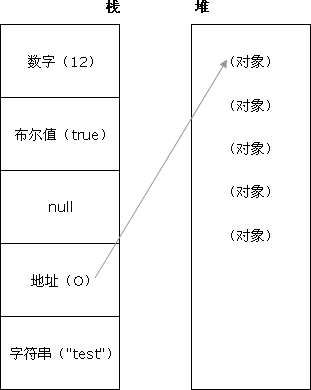
\includegraphics[scale=0.5]{js_value.png}
\vspace{-10pt}
\caption{Stack \& Heap}
\label{stack_heap}
\end{figure}

如果一个值是引用类型的,那么它的存储空间将从堆中分配。由于引用值的大小会改变,所以不能把它放在栈中,否则会降低变量查寻的速度。相反,放在变量的栈空间中的值是该对象存储在堆中的地址。地址的大小是固定的,所以把它存储在栈中对变量性能无任何负面影响。

在许多语言中,字符串都被看作引用类型,而非原始类型,因为字符串的长度是可变的,但是ECMAScript 打破了这一传统。

ECMAScript 有 5 种原始类型(primitive type),即 Undefined、Null、Boolean、Number 和 String。

ECMA-262 把术语类型(type)定义为值的一个集合,每种原始类型定义了它包含的值的范围及其字面量表示形式。




JavaScript 拥有动态类型,这意味着相同的变量可用作不同的类型:

\begin{lstlisting}[language=JavaScript]
var x                // x 为 undefined
var x = 6;           // x 为数字
var x = "Bill";      // x 为字符串
\end{lstlisting}

ECMAScript 有 5 种原始类型(primitive type),即 Undefined、Null、Boolean、Number 和 String。

声明新变量时,可以使用关键词 "new" 来声明其类型:

\begin{lstlisting}[language=JavaScript]
var carname=new String;
var x=      new Number;
var y=      new Boolean;
var cars=   new Array;
var person= new Object;
\end{lstlisting}

JavaScript 中的所有事物都是对象:字符串、数字、数组、日期等,因此JavaScript 变量均为对象,当声明一个变量时,就创建了一个新的对象。












\chapter{Primitive Types}




\section{Typeof Operator}


ECMAScript 提供了 typeof 运算符来判断一个值是否在某种类型的范围内,可以typeof运算符判断一个值是否表示一种原始类型:如果它是原始类型,还可以判断它表示哪种原始类型。

typeof 运算符有一个参数,即要检查的变量或值。例如:



\begin{lstlisting}[language=JavaScript]
var sTemp = "test string";
alert (typeof sTemp);    //输出 "string"
alert (typeof 86);    //输出 "number"
\end{lstlisting}



对变量或值调用 typeof 运算符将返回下列值之一:

\begin{compactitem}
\item undefined - 如果变量是 Undefined 类型的
\item boolean - 如果变量是 Boolean 类型的
\item number - 如果变量是 Number 类型的
\item string - 如果变量是 String 类型的
\item object - 如果变量是一种引用类型或 Null\footnote{至于为什么 typeof 运算符对于 null 值会返回 "Object"。这实际上是 JavaScript 最初实现中的一个错误,然后被 ECMAScript 沿用了。现在,null 被认为是对象的占位符,从而解释了这一矛盾,但从技术上来说,它仍然是原始值。}类型的
\end{compactitem}





\section{Undefined}


Undefined 类型只有一个值,即 undefined。当声明的变量未初始化时,该变量的默认值是 undefined。



\begin{lstlisting}[language=JavaScript]
var oTemp;
var sTemp = "test string";
alert (typeof sTemp);    	//输出 "string"
alert(typeof oTemp);	//输出"undefined"
alert (typeof 86);    		//输出 "number"
alert(oTemp == undefined);
\end{lstlisting}

虽然,值 undefined 并不同于未定义的值。但是,typeof 运算符并不真正区分这两种值。考虑下面的代码:


\begin{lstlisting}[language=JavaScript]
var oTemp;

alert(typeof oTemp);  //输出 "undefined"
alert(typeof oTemp2);  //输出 "undefined"
\end{lstlisting}


前面的代码对两个变量输出的都是 "undefined",即使只有变量 oTemp2 从未被声明过。如果对 oTemp2 使用除 typeof 之外的其他运算符的话,会引起错误,因为其他运算符只能用于已声明的变量上。例如,下面的代码将引发错误:

\begin{lstlisting}[language=JavaScript]
var oTemp;
alert(oTemp2 == undefined);
\end{lstlisting}

另外,当函数无明确返回值时,返回的也是值 "undefined",如下所示:



\begin{lstlisting}[language=JavaScript]
function testFunc() {
}

alert(testFunc() == undefined);  //输出 "true"
\end{lstlisting}


\section{Null}


另一种只有一个值的类型是 Null,它只有一个专用值 null,即它的字面量。值 undefined 实际上是从值 null 派生来的,因此 ECMAScript 把它们定义为相等的,Undefined 这个值表示变量不含有值,可以通过将变量的值设置为 null 来清空变量。



\begin{lstlisting}[language=JavaScript]
cars=null;
person=null;
alert(typeof cars);	//输出“object”
alert(typeof persion);	//输出“object”
alert(null == undefined);  //输出 "true"
\end{lstlisting}

尽管这两个值相等,但它们的含义不同。undefined 是声明了变量但未对其初始化时赋予该变量的值,null 则用于表示尚未存在的对象。如果函数或方法要返回的是对象,那么找不到该对象时,返回的通常是 null。





\section{Boolean}


Boolean 类型是 ECMAScript 中最常用的类型之一,它有两个值 true 和 false (即两个 Boolean 字面量),常用在条件测试中。。


即使 false 不等于 0,0 也可以在必要时被转换成 false,这样在 Boolean 语句中使用两者都是安全的。


\begin{lstlisting}[language=JavaScript]
var bFound = true;
var bLost = false;
\end{lstlisting}





\section{Number}

ECMA-262 中定义的最特殊的类型是 Number 类型,JavaScript 只有一种数字类型,数字可以带小数点,也可以不带。

\begin{lstlisting}[language=JavaScript]
var x1=34.00;      //使用小数点来写
var x2=34;         //不使用小数点来写
\end{lstlisting}



Number类型既可以表示 32 位的整数,还可以表示 64 位的浮点数。直接输入的(而不是从另一个变量访问的)任何数字都被看做 Number 类型的字面量。例如,下面的代码声明了存放整数值的变量,它的值由字面量 86 定义:


\begin{lstlisting}[language=JavaScript]
var iNum = 86;
alert(iNum == number);
alert (typeof 86);    		//输出 "number"
\end{lstlisting}


\subsection{Octal Number}


整数也可以被表示为八进制(以 8 为底)或十六进制(以 16 为底)的字面量\footnote{尽管所有整数都可以表示为八进制或十六进制的字面量,但所有数学运算返回的都是十进制结果。}。八进制字面量的首数字必须是 0,其后的数字可以是任何八进制数字(0-7),如下面的代码所示:



\begin{lstlisting}[language=JavaScript]
var iNum = 86;		//十进制数86
var iNum = 070;  	//070 等于十进制的 56
\end{lstlisting}


\subsection{Hex Number}



要创建十六进制的字面量,首位数字必须为 0,后面接字母 x,然后是任意的十六进制数字(0 到 9 和 A 到 F)。这些字母可以是大写的,也可以是小写的。例如:



\begin{lstlisting}[language=JavaScript]
var iNum = 0x1f;  //0x1f 等于十进制的 31
var iNum = 0xAB;  //0xAB 等于十进制的 171
\end{lstlisting}


\subsection{Float Number}


要定义浮点值,必须包括小数点和小数点后的一位数字(例如,用 1.0 而不是 1)。这被看作浮点数字面量。例如:


\begin{lstlisting}[language=JavaScript]
var iNum = 86;		//十进制数86
var iNum = 070;  	//070 等于十进制的 56
var iNum = 0x1f;  	//0x1f 等于十进制的 31
var iNum = 0xAB;  	//0xAB 等于十进制的 171
var fNum = 5.0;		//浮点数5.0
\end{lstlisting}

对于浮点字面量的有趣之处在于,用它进行计算前,真正存储的是字符串。


\subsection{Infinity}


对于非常大或非常小的数,可以用科学计数法表示浮点数,从而可以把一个数表示为数字(包括十进制数字)加 e(或 E),后面加乘以 10 的倍数。例如:


\begin{lstlisting}[language=JavaScript]
var iNum = 86;			//十进制数86
var iNum = 070;  		//070 等于十进制的 56
var iNum = 0x1f;  		//0x1f 等于十进制的 31
var iNum = 0xAB;  		//0xAB 等于十进制的 171
var fNum = 5.0;			//浮点数5.0
var fNum = 5.618e7;	//浮点数 56180000
var y=123e5;      // 12300000
var z=123e-5;     // 0.00123
\end{lstlisting}

该符号表示的是数 56180000。把科学计数法转化成计算式就可以得到该值:$\text{5.618}\times \text{10}^{\text{7}}$。


\subsection{Scientific notation}




也可以用科学计数法表示非常小的数,例如 0.00000000000000008 可以表示为$\text{8}\times e^{-\text{17}}$(这里,10 被升到 -17 次幂,意味着需要被 10 除 17 次)。ECMAScript 默认把具有 6 个或 6 个以上前导 0 的浮点数转换成科学计数法。

也可用 64 位 IEEE 754 形式存储浮点值,这意味着十进制值最多可以有 17 个十进制位。17 位之后的值将被裁去,从而造成一些小的数学误差。


几个特殊值也被定义为 Number 类型,其中前两个是 Number.MAX\_VALUE 和 Number.MIN\_VALUE,它们定义了 Number 值集合的外边界。所有 ECMAScript 数都必须在这两个值之间,不过计算生成的数值结果可以不落在这两个值之间。

当计算生成的数大于 Number.MAX\_VALUE 时,它将被赋予值 Number.POSITIVE\_INFINITY,意味着不再有数字值。同样,生成的数值小于 Number.MIN\_VALUE 的计算也会被赋予值 Number.NEGATIVE\_INFINITY,也意味着不再有数字值。如果计算返回的是无穷大值,那么生成的结果不能再用于其他计算。

事实上,有专门的值表示无穷大,(如你猜到的)即 Infinity。Number.POSITIVE\_INFINITY 的值为 Infinity。Number.NEGATIVE\_INFINITY 的值为 -Infinity。

由于无穷大数可以是正数也可以是负数,所以可用一个方法判断一个数是否是有穷的(而不是单独测试每个无穷数)。可以对任何数调用 isFinite() 方法,以确保该数不是无穷大。例如:



\begin{lstlisting}[language=JavaScript]
var iResult = iNum * some_really_large_number;

if (isFinite(iResult)) {
    alert("finite");
}

else {
    alert("infinite");
}
\end{lstlisting}


\subsection{NaN}


最后一个特殊值是 NaN,表示非数(Not a Number)。NaN 是个奇怪的特殊值。一般说来,这种情况发生在类型(String、Boolean 等)转换失败时。例如,要把单词 blue 转换成数值就会失败,因为没有与之等价的数值。与无穷大一样,NaN 也不能用于算术计算。NaN 的另一个奇特之处在于,它与自身不相等,这意味着下面的代码将返回 false:


\begin{lstlisting}[language=JavaScript]
alert(NaN == NaN);  //输出 "false"
\end{lstlisting}

出于这个原因,不推荐使用 NaN 值本身。函数 isNaN() 会做得相当好:

\begin{lstlisting}[language=JavaScript]
alert(isNaN("blue"));  //输出 "true"
alert(isNaN("666"));  //输出 "false"
\end{lstlisting}

JavaScript最早是在HTML网页上使用,用来给HTML网页增加动态功能,比如JavaScript 常用于验证用户的输入,比如在下面的例子中,如果输入值不是数字,浏览器会弹出提示框。



\begin{lstlisting}[language=HTML]
<input id="demo" type="text">

<script>
function myFunction()
{
var x=document.getElementById("demo").value;
if(x==""||isNaN(x))
	{
	alert("Not Numeric");
	}
}
</script>

<button type="button" onclick="myFunction()">点击这里</button>
\end{lstlisting}



\section{String}

JavaScript 变量还能保存其他数据类型,比如文本值 (name="Bill Gates"),这又称为String类型。

String 类型的独特之处在于,它是唯一没有固定大小的原始类型,可以用字符串存储 0 或更多的 Unicode 字符,由16 位整数表示。

字符串中每个字符都有特定的位置,首字符从位置 0 开始,第二个字符在位置 1,依此类推。这意味着字符串中的最后一个字符的位置一定是字符串的长度减 1:

\begin{figure}[!h]
\centering
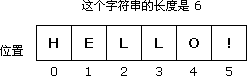
\includegraphics[scale=0.5]{js_string.png}
\caption{EMAScript String 类型}
\label{js_string}
\end{figure}

JavaScript字符串字面量是由双引号(")或单引号(')声明的,字符串可以是引号中的任意文本,因此当向变量赋的值是数值时,不要使用引号。如果用引号包围数值,该值会被作为文本来处理。

由于 ECMAScript 没有字符类型,所以JavaScript可使用这两种表示法中的任何一种。Java 则是用双引号声明字符串,用单引号声明字符。例如,下面的两行JavaScript代码都有效:


\begin{lstlisting}[language=JavaScript]
var sColor1 = "red";
var sColor2 = 'red';
\end{lstlisting}



可以在字符串中使用引号,只要不匹配包围字符串的引号即可:


\begin{lstlisting}[language=JavaScript]
var answer="Nice to meet you!";
var answer="He is called 'Bill'";
var answer='He is called "Bill"';
\end{lstlisting}




String 类型还包括几种字符字面量,Java、C 和 Perl 的开发者应该对此非常熟悉,在下面的表格中列出了 ECMAScript 的字符字面量:

\begin{longtable}{|m{50pt}|m{300pt}|}
%head
\multicolumn{2}{r}{}
\tabularnewline\hline
字面量	&含义
\endhead
%endhead

%firsthead
\caption{ECMAScript 的字符字面量}\\
\hline
字面量	&含义
\endfirsthead
%endfirsthead

%foot
\multicolumn{2}{r}{}
\endfoot
%endfoot

%lastfoot
\endlastfoot
%endlastfoot

\hline
\verb|\n|	&换行\\
\hline
\verb|\t|	&制表符\\
\hline
\verb|\b|	&空格\\
\hline
\verb|\r|	&回车\\
\hline
\verb|\f|	&换页符\\
\hline
\verb|\\|	&反斜杠\\
\hline
\verb|\'|	&单引号\\
\hline
\verb|\"|	&双引号\\
\hline
\verb|\0nnn|	&八进制代码 nnn 表示的字符(n 是 0 到 7 中的一个八进制数字)\\
\hline
\verb|\xnn|	&十六进制代码 nn 表示的字符(n 是 0 到 F 中的一个十六进制数字)\\
\hline
\verb|\unnnn|	&十六进制代码 nnnn 表示的 Unicode 字符(n 是 0 到 F 中的一个十六进制数字)\\
\hline

\end{longtable}



\section{Array}

下面的代码创建名为 cars 的数组:

\begin{lstlisting}[language=JavaScript]
var cars=new Array();
cars[0]="Audi";
cars[1]="BMW";
cars[2]="Volvo";
\end{lstlisting}

或者 (condensed array):


\begin{lstlisting}[language=JavaScript]
var cars=new Array("Audi","BMW","Volvo");
\end{lstlisting}

或者 (literal array):

\begin{lstlisting}[language=JavaScript]
var cars=["Audi","BMW","Volvo"];
\end{lstlisting}

数组下标是基于零的,所以第一个项目是 [0],第二个是 [1],以此类推。


\chapter{Type Conversion}

所有程序设计语言最重要的特征之一是具有进行类型转换的能力,ECMAScript 给开发者提供了大量简单的类型转换方法。

大部分类型具有进行简单转换的方法,还有几个全局方法可以用于更复杂的转换。无论哪种情况,在 ECMAScript 中,类型转换都是简短的一步操作。


\section{String}

ECMAScript 的 Boolean 值、数字和字符串的原始值的有趣之处在于它们是伪对象,这意味着它们实际上具有属性和方法。例如,要获得字符串的长度,可以采用下面的代码:

\begin{lstlisting}[language=JavaScript]
var sColor = "red";
alert(sColor.length);	//输出 "3"
\end{lstlisting}


尽管 "red" 是原始类型的字符串,它仍然具有属性 length,用于存放字符串的大小。总而言之,3 种主要的原始类型 Boolean 值、数字和字符串都有 toString() 方法,可以把它们的值转换成字符串。

ECMAScript 定义所有对象都有 toString() 方法,无论它是伪对象,还是真对象。因为 String 类型属于伪对象,所以它一定有 toString() 方法。


\subsection{Boolean}


Boolean 类型的 toString() 方法只是输出 "true" 或 "false",结果由变量的值决定:


\begin{lstlisting}[language=JavaScript]
var bFound = false;
alert(bFound.toString());	//输出 "false"
\end{lstlisting}




\subsection{Number}

Number 类型的 toString() 方法比较特殊,它有两种模式,即默认模式和基模式。采用默认模式,toString() 方法只是用相应的字符串输出数字值(无论是整数、浮点数还是科学计数法),如下所示:


\begin{lstlisting}[language=JavaScript]
var iNum1 = 10;
var iNum2 = 10.0;
alert(iNum1.toString());	//输出 "10"
alert(iNum2.toString());	//输出 "10"
\end{lstlisting}



在默认模式中,无论最初采用什么表示法声明数字,Number 类型的 toString() 方法返回的都是数字的十进制表示。因此,以八进制或十六进制字面量形式声明的数字输出的都是十进制形式的。


采用 Number 类型的 toString() 方法的基模式,可以用不同的基输出数字,基只是要转换成的基数的另一种加法而已,它是 toString() 方法的参数,例如二进制的基是 2,八进制的基是 8,十六进制的基是 16。



\begin{lstlisting}[language=JavaScript]
var iNum = 10;
alert(iNum.toString(2));	//输出 "1010"
alert(iNum.toString(8));	//输出 "12"
alert(iNum.toString(16));	//输出 "A"
\end{lstlisting}


在上面的示例中,以 3 种不同的形式输出了数字 10,即二进制形式、八进制形式和十六进制形式\footnote{对数字调用 toString(10) 与调用 toString() 相同,它们返回的都是该数字的十进制形式。}。

HTML 采用十六进制表示每种颜色,在 HTML 中处理数字时这种功能非常有用。


\begin{compactitem}
\item arrayObject.toString()
\item booleanObject.toString()
\item dateObject.toString()
\item NumberObject.toString()
\item stringObject.toString()
\end{compactitem}



\section{Number}


ECMAScript 提供了两种把非数字的原始值转换成数字的方法,即 parseInt() 和 parseFloat(),其中前者把值转换成整数,后者把值转换成浮点数。只有对 String 类型调用这些方法,它们才能正确运行,对其他类型返回的都是 NaN。


\subsection{parseInt()}

在判断字符串是否是数字值前,parseInt() 和 parseFloat() 都会仔细分析该字符串。

parseInt() 方法首先查看位置 0 处的字符,判断它是否是个有效数字;如果不是,该方法将返回 NaN,不再继续执行其他操作。但如果该字符是有效数字,该方法将查看位置 1 处的字符,进行同样的测试。这一过程将持续到发现非有效数字的字符为止,此时 parseInt() 将把该字符之前的字符串转换成数字。例如,如果要把字符串 "12345red" 转换成整数,那么 parseInt() 将返回 12345,因为当它检查到字符 r 时,就会停止检测过程。

字符串中包含的数字字面量会被正确转换为数字,比如 "0xA" 会被正确转换为数字 10。不过,字符串 "22.5" 将被转换成 22,因为对于整数来说,小数点是无效字符。



\begin{lstlisting}[language=JavaScript]
var iNum1 = parseInt("12345red");	//返回 12345
var iNum1 = parseInt("0xA");	//返回 10
var iNum1 = parseInt("56.9");	//返回 56
var iNum1 = parseInt("red");	//返回 NaN
\end{lstlisting}

parseInt() 方法还有基模式,可以把二进制、八进制、十六进制或其他任何进制的字符串转换成整数(默认模式是十进制)。基是由 parseInt() 方法的第二个参数指定的,所以如果要解析十六进制的值,需如下调用 parseInt() 方法:


\begin{lstlisting}[language=JavaScript]
var iNum1 = parseInt("10", 2);	//返回 2
var iNum2 = parseInt("10", 8);	//返回 8
var iNum3 = parseInt("10", 10);	//返回 10
var iNum1 = parseInt("AF", 16);	//返回 175
\end{lstlisting}

如果十进制数包含前导 0,那么最好采用基数 10,这样才不会意外地得到八进制的值。例如:


\begin{lstlisting}[language=JavaScript]
var iNum1 = parseInt("010");	//返回 8
var iNum2 = parseInt("010", 8);	//返回 8
var iNum3 = parseInt("010", 10);	//返回 10
\end{lstlisting}

在这段代码中,两行代码都把字符 "010" 解析成一个数字。第一行代码把这个字符串看作八进制的值,解析它的方式与第二行代码(声明基数为 8)相同。最后一行代码声明基数为 10,所以 iNum3 最后等于 10。




\subsection{parseFloat()}

parseFloat() 方法与 parseInt() 方法的处理方式相似,从位置 0 开始查看每个字符,直到找到第一个非有效的字符为止,然后把该字符之前的字符串转换成整数。

不过,对于这个方法来说,第一个出现的小数点是有效字符。如果有两个小数点,第二个小数点将被看作无效的。parseFloat() 会把这个小数点之前的字符转换成数字。这意味着字符串 "11.22.33" 将被解析成 11.22。

使用 parseFloat() 方法的另一不同之处在于,字符串必须以十进制形式表示浮点数,而不是用八进制或十六进制。该方法会忽略前导 0,所以八进制数 0102 将被解析为 102。对于十六进制数 0xA,该方法将返回 NaN,因为在浮点数中,x 不是有效字符\footnote{注释:经测试,具体的浏览器实现会返回 0,而不是 NaN。}。

此外,parseFloat() 方法也没有基模式。



\begin{lstlisting}[language=JavaScript]
var fNum1 = parseFloat("12345red");	//返回 12345
var fNum2 = parseFloat("0xA");	//返回 NaN
var fNum3 = parseFloat("11.2");	//返回 11.2
var fNum4 = parseFloat("11.22.33");	//返回 11.22
var fNum5 = parseFloat("0102");	//返回 102
var fNum1 = parseFloat("red");	//返回 NaN
\end{lstlisting}



\section{Type Casting}


可以使用强制类型转换(type casting)\footnote{cast 有“铸造”之意,很贴合“强制转换”的意思。}来处理转换值的类型。使用强制类型转换可以访问特定的值,即使它是另一种类型的。

ECMAScript 中可用的 3 种强制类型转换如下:

\begin{compactitem}
\item Boolean(value) - 把给定的值转换成 Boolean 型;
\item Number(value) - 把给定的值转换成数字(可以是整数或浮点数);
\item String(value) - 把给定的值转换成字符串;
\end{compactitem}

用这三个函数之一转换值,将创建一个新值,存放由原始值直接转换成的值,但这会造成意想不到的后果。


\subsection{Boolean()}



当要转换的值是至少有一个字符的字符串、非 0 数字或对象时,Boolean() 函数将返回 true。如果该值是空字符串、数字 0、undefined 或 null,它将返回 false。可以用下面的代码测试 Boolean 型的强制类型转换:


\begin{lstlisting}[language=JavaScript]
var b1 = Boolean("");		//false - 空字符串
var b2 = Boolean("hello");		//true - 非空字符串
var b1 = Boolean(50);		//true - 非零数字
var b1 = Boolean(null);		//false - null
var b1 = Boolean(0);		//false - 零
var b1 = Boolean(new object());	//true - 对象
\end{lstlisting}



\subsection{Number()}

Number() 函数的强制类型转换与 parseInt() 和 parseFloat() 方法的处理方式相似,只是它转换的是整个值,而不是部分值。


parseInt() 和 parseFloat() 方法只转换第一个无效字符之前的字符串,因此 "1.2.3" 将分别被转换为 "1" 和 "1.2"。用 Number() 进行强制类型转换时,"1.2.3" 将返回 NaN,因为整个字符串值不能转换成数字。如果字符串值能被完整地转换,Number() 将判断是调用 parseInt() 方法还是 parseFloat() 方法。

下表说明了对不同的值调用 Number() 方法会发生的情况:

\begin{longtable}{|m{150pt}|m{100pt}|}
%head
\multicolumn{2}{r}{}
\tabularnewline\hline
用法	&结果
\endhead
%endhead

%firsthead
\hline
用法	&结果
\endfirsthead
%endfirsthead

%foot
\multicolumn{2}{r}{}
\endfoot
%endfoot

%lastfoot
\endlastfoot
%endlastfoot

\hline
Number(false)	&0\\
\hline
Number(true)	&1\\
\hline
Number(undefined)	&NaN\\
\hline
Number(null)	&0\\
\hline
Number("1.2")	&1.2\\
\hline
Number("12")	&12\\
\hline
Number("1.2.3")	&NaN\\
\hline
Number(new object())	&NaN\\
\hline
Number(50)	&50\\
\hline

\end{longtable}





\subsection{String()}

强制类型转换方法 String() 是最简单的,因为它可把任何值转换成字符串。


要执行这种强制类型转换,只需要调用作为参数传递进来的值的 toString() 方法,即把 12 转换成 "12",把 true 转换成 "true",把 false 转换成 "false",以此类推。

强制转换成字符串和调用 toString() 方法的唯一不同之处在于,对 null 和 undefined 值强制类型转换可以生成字符串而不引发错误:


\begin{lstlisting}[language=JavaScript]
var s1 = String(null);	//"null"
var oNull = null;
var s2 = oNull.toString();	//会引发错误
\end{lstlisting}

在处理 ECMAScript 这样的弱类型语言时,强制类型转换非常有用,不过应该确保使用值的正确。




\chapter{Reference Types}

引用类型通常叫做类(class)\footnote{注意:从传统意义上来说,ECMAScript 并不真正具有类。事实上,除了说明不存在类,在 ECMA-262 中根本没有出现“类”这个词。ECMAScript 定义了“对象定义”,逻辑上等价于其他程序设计语言中的类。},也就是说,遇到引用值,所处理的就是对象。

JavaScript 是面向对象的语言,但 JavaScript 不使用类,实际上JavaScript 基于 prototype,而不是基于类的。

JavaScript的对象是拥有属性和方法的特殊数据类型。其中,属性是与对象相关的值,而方法是能够在对象上执行的动作。

可以通过如下的语法访问对象的属性,调用对象的方法,而且上面列出的每种属性和方法都会被其他对象覆盖。

\begin{lstlisting}[language=JavaScript]
objectName.propertyName
objectName.methodName()
\end{lstlisting}

如果要访问字符串对象“Hello world!”的length属性,并且把将其转换为大写,可以通过如下的代码:


\begin{lstlisting}[language=JavaScript]
var message="Hello World!";
var x=message.length;
var y=message.toUpperCase();
alert(x);
alert(y);
\end{lstlisting}

JavaScript 中的所有事物都是对象:字符串、数字、数组、日期等,而且JavaScript 提供多个内建对象,比如 String、Date、Array 等。

此外,JavaScript 允许自定义对象,创建新对象有两种不同的方法:

\begin{compactitem}
\item 定义并创建对象的实例
\item 使用函数来定义对象,然后创建新的对象实例
\end{compactitem}





举例来说,汽车就是现实生活中的对象,其中汽车的属性有:



\begin{lstlisting}[language=JavaScript]
var car = new Object();
car.name=Fiat
car.model=500
car.weight=850kg
car.color=white 
\end{lstlisting}

也可以使用替代语法(使用对象 literals),即:

\begin{lstlisting}[language=JavaScript]
car = {name:"Fiat", model:"500", weight:"850kg",color:"white"};
\end{lstlisting}

\section{Object Constructor}

使用函数(对象构造器)来构造对象的语法如下:



\begin{lstlisting}[language=JavaScript]
function car(name, model, weight, color){
  this.name = name;
  this.model = model;
  this.weight = weight;
  this.color = color;
}
\end{lstlisting}

通过对象构造器,就可以创建新的对象实例,代码如下:

\begin{lstlisting}[language=JavaScript]
var car1 = new car("Fiat", model:"500", weight:"850kg",color:"white");
\end{lstlisting}

可以通过为对象赋值,向已有对象添加新属性,,代码如下:


\begin{lstlisting}[language=JavaScript]
car.name = "Fiat";
car.model = "500";
car.weight = "850kg";
car.color = "white";
\end{lstlisting}




汽车的属性包括名称、型号、重量、颜色等,而且所有汽车都有这些属性,但是每款车的属性都不尽相同。

方法只不过是附加在对象上的函数,下面是在构造器函数内部定义对象的方法:

\begin{lstlisting}[language=JavaScript]
function car(name, model, weight, color){
  this.name = name;
  this.model = model;
  this.weight = weight;
  this.color = color;

  this.start = start;
  function start(){
  
  }
  ...
}
\end{lstlisting}



汽车的方法有:


\begin{lstlisting}[language=JavaScript]
var car = new Object();
car.start()
car.drive()
car.brake()
\end{lstlisting}

汽车的方法可以是启动、驾驶、刹车等。所有汽车都拥有这些方法,但是它们被执行的时间都不尽相同。

另一个对象构造的例子如下:

\begin{lstlisting}[language=JavaScript]
function person(firstname,lastname,age,eyecolor){
  this.firstname=firstname;
  this.lastname=lastname;
  this.age=age;
  this.eyecolor=eyecolor;

  this.changeName=changeName;
  function changeName(name){
    this.lastname=name;
  }
}
\end{lstlisting}


其中,changeName() 函数 name 的值赋给 person 的 lastname 属性,下面是使用函数对对象执行操作的示例:


\begin{lstlisting}[language=JavaScript]
var myFather=new person("Jim","Green",30,"blue");
var myMother=new person("Meimei","Han",28,"black");
myMother.changeName("Jane");
\end{lstlisting}

JavaScript for...in 语句循环可以遍历对象的属性,for...in 循环中的代码块将针对每个属性执行一次,语法如下:

\begin{lstlisting}[language=JavaScript]
for (对象中的变量){
  要执行的代码
}
\end{lstlisting}

下面的示例将循环遍历对象的属性:

\begin{lstlisting}[language=JavaScript]
var person={fname:"Jim",lname:"Green",age:30};

for (x in person){
  txt=txt + person[x];
}
\end{lstlisting}




\section{Object}

在 JavaScript 中,对象是数据(变量),拥有属性和方法,当声明一个 JavaScript 变量时,实际上就已经创建了一个对象,比如:

\begin{lstlisting}[language=JavaScript]
var u;
var bFound = true;
var iNum = 2013;
var cars=new Array("Audi","BMW","Volvo");
var sTxt = "Hello";
\end{lstlisting}

字符串对象拥有内建的属性 length,因此对于上面的字符串来说,length 的值是 5,同时字符串对象同时拥有若干个内建的方法。

在面向对象的语言中,属性和方法常被称为对象的成员,以上例中的sTxt字符串变量为例,就是:

\begin{lstlisting}[language=JavaScript]
txt.length=5
txt.indexOf()
txt.replace()
txt.search()
\end{lstlisting}


JavaScript 中的几乎所有事物都是对象:字符串、数字、数组、日期、函数等,可以由 new 运算符加上要实例化的对象的名字创建。例如,下面的代码创建 Object 对象的实例:


\begin{lstlisting}[language=JavaScript]
var o = new Object();
\end{lstlisting}

创建新 JavaScript 对象有很多不同的方法,并且还可以向已存在的对象添加属性和方法。下面创建名为 "person" 的对象,并为其添加了四个属性:

\begin{lstlisting}[language=JavaScript]
var person = new Object();
person.firstname="Jim";
person.lastname="Green";
person.age=30;
person.eyecolor="green";
\end{lstlisting}



这种语法与 Java 语言的相似,不过当有不止一个参数时,ECMAScript 要求使用括号。如果没有参数,如以下代码所示,括号可以省略\footnote{注意:尽管括号不是必需的,但是为了避免混乱,最好使用括号。}:

\begin{lstlisting}[language=JavaScript]
var o = new Object;
\end{lstlisting}

Object 对象自身用处不大,只是ECMAScript 中的 Object 对象与 Java 中的 java.lang.Object 相似,ECMAScript 中的所有对象都由这个对象继承而来,Object 对象中的所有属性和方法都会出现在其他对象中,所以理解了 Object 对象,就可以更好地理解其他对象。

Object 对象具有下列属性:

\begin{compactitem}
\item constructor
对创建对象的函数的引用(指针)。对于 Object 对象,该指针指向原始的 Object() 函数。
\item Prototype
对该对象的对象原型的引用。对于所有的对象,它默认返回 Object 对象的一个实例。
\end{compactitem}




Object 对象具有下列方法:

\begin{compactitem}
\item hasOwnProperty(property)
判断对象是否有某个特定的属性。必须用字符串指定该属性。(例如,o.hasOwnProperty("name"))
\item IsPrototypeOf(object)
判断该对象是否为另一个对象的原型。
\item PropertyIsEnumerable
判断给定的属性是否可以用 for...in 语句进行枚举。
\item ToString()
返回对象的原始字符串表示。对于 Object 对象,ECMA-262 没有定义这个值,所以不同的 ECMAScript 实现具有不同的值。
\item ValueOf()
返回最适合该对象的原始值。对于许多对象,该方法返回的值都与 ToString() 的返回值相同。
\end{compactitem}



对象由花括号分隔。在括号内部,对象的属性以名称和值对的形式 (name : value) 来定义,属性由逗号分隔:


\begin{lstlisting}[language=JavaScript]
var person={firstname:"Jim", lastname:"Green", id:1002};
\end{lstlisting}

上面例子中的对象 (person) 有三个属性:firstname、lastname 以及 id,空格和折行无关紧要。

JavaScript对象声明可横跨多行:


\begin{lstlisting}[language=JavaScript]
var person={
firstname : "Jim",
lastname  : "Green",
id        :  1002
};
\end{lstlisting}

对象属性有两种寻址方式:

\begin{lstlisting}[language=JavaScript]
name=person.lastname;
name=person["lastname"];
\end{lstlisting}


\section{Boolean Object}

Boolean 对象是 Boolean 原始类型的引用类型,用于将非逻辑值转换为逻辑值(true 或者 false)。


可以将 Boolean 对象理解为一个产生逻辑值的对象包装器,如果要创建 Boolean 对象,只需要传递 Boolean 值作为参数:



\begin{lstlisting}[language=JavaScript]
var oBooleanObject = new Boolean(true);
\end{lstlisting}



Boolean 对象将覆盖 Object 对象的 ValueOf() 方法,返回原始值,即 true 和 false。ToString() 方法也会被覆盖,返回字符串 "true" 或 "false"。但是,在 ECMAScript 中很少使用 Boolean 对象,即使使用,也不易理解。问题通常出现在 Boolean 表达式中使用 Boolean 对象时,例如:



\begin{lstlisting}[language=JavaScript]
var oFalseObject = new Boolean(false);
var bResult = oFalseObject && true;	//输出 true
\end{lstlisting}



在这段代码中,用 false 值创建 Boolean 对象,然后用这个值与原始值 true 进行 AND 操作。

在 Boolean 运算中,false 和 true 进行 AND 操作的结果是 false。不过,在上述这行代码中,计算的是 oFalseObject,而不是它的值 false\footnote{注意:虽然你应该了解 Boolean 对象的可用性,不过最好还是使用 Boolean 原始值,避免发生这一节提到的问题。}。

在 Boolean 表达式中,所有对象都会被自动转换为 true,所以 oFalseObject 的值是 true。然后 true 再与 true 进行 AND 操作,结果为 true。

如果逻辑对象无初始值或者其值为 0、-0、null、""、false、undefined 或者 NaN,那么对象的值为 false。否则,其值为 true(即使当自变量为字符串 "false" 时)。

下面的所有的代码行均会创建初始值为 false 的 Boolean 对象。


\begin{lstlisting}[language=JavaScript]
var myBoolean=new Boolean();
var myBoolean=new Boolean(0);
var myBoolean=new Boolean(null);
var myBoolean=new Boolean("");
var myBoolean=new Boolean(false);
var myBoolean=new Boolean(NaN);
\end{lstlisting}

下面的所有的代码行均会创初始值为 true 的 Boolean 对象:


\begin{lstlisting}[language=JavaScript]
var myBoolean=new Boolean(1);
var myBoolean=new Boolean(true);
var myBoolean=new Boolean("true");
var myBoolean=new Boolean("false");
var myBoolean=new Boolean("Jim Green");
\end{lstlisting}

\section{Number Object}


Number 对象是 Number 原始类型的引用类型。JavaScript 只有一种数字类型,可以使用也可以不使用小数点来书写数字,极大或极小的数字可通过科学(指数)计数法来写。

要创建 Number 对象,采用下列代码:

\begin{lstlisting}[language=JavaScript]
var oNumberObject = new Number(value);
var oNumberObject = Number(value);
\end{lstlisting}


JavaScript 不是类型语言。与许多其他编程语言不同,JavaScript 不定义不同类型的数字,比如整数、短、长、浮点等,JavaScript 中的所有数字都存储为根为 10 的 64 位(8 比特)的浮点数。

整数(不使用小数点或指数计数法)最多为 15 位,小数的最大位数是 17,但是浮点运算并不总是 100\% 准确。同样,如果前缀为 0,则 JavaScript 会把数值常量解释为八进制数,如果前缀为 0 和 "x",则解释为十六进制数。

Number对象的属性包括:

\begin{compactitem}
\item MAX\_VALUE
\item MIN\_VALUE
\item NEGATIVE\_INFINITIVE
\item POSITIVE\_INFINITIVE
\item NaN
\item prototype
\item constructor
\end{compactitem}

所有特殊值都是 Number 对象的静态属性,比如Number.MAX\_VALUE,要得到数字对象的 Number 原始值,可以使用 valueOf() 方法:


\begin{lstlisting}[language=JavaScript]
var iNumber = oNumberObject.valueOf();
\end{lstlisting}

当然,Number 类也有 toString() 方法,而且除了从 Object 对象继承的标准方法外,Number 对象还有几个处理数值的专用方法。

\begin{compactitem}
\item toExponential()
\item toFixed()
\item toPrecision()
\item toString()
\item valueOf()
\end{compactitem}



\subsection{toFixed()}

toFixed() 方法返回的是具有指定位数小数的数字的字符串表示。例如:


\begin{lstlisting}[language=JavaScript]
var oNumberObject = new Number(68);
alert(oNumberObject.toFixed(2));  //输出 "68.00"
\end{lstlisting}

在这里,toFixed() 方法的参数是 2,说明应该显示两位小数。该方法返回 "68.00",空的字符串位由 0 来补充。对于处理货币的应用程序,该方法非常有用。toFixed() 方法能表示具有 0 到 20 位小数的数字,超过这个范围的值会引发错误。

\subsection{toExponential()}

与格式化数字相关的另一个方法是 toExponential(),它返回的是用科学计数法表示的数字的字符串形式。

与 toFixed() 方法相似,toExponential() 方法也有一个参数,指定要输出的小数的位数。例如:

\begin{lstlisting}[language=JavaScript]
var oNumberObject = new Number(68);
alert(oNumberObject.toExponential(1));  //输出 "6.8e+1"
\end{lstlisting}

这段代码的结果是 "6.8e+1",如果不知道要用哪种形式(预定形式或指数形式)表示数字,可以用 toPrecision() 方法。




\subsection{toPrecision()}




toPrecision() 方法根据最有意义的形式来返回数字的预定形式或指数形式。它有一个参数,即用于表示数的数字总数(不包括指数)。例如,


\begin{lstlisting}[language=JavaScript]
var oNumberObject = new Number(68);
alert(oNumberObject.toPrecision(1));  //输出 "7e+1"
\end{lstlisting}

这段代码的任务是用一位数字表示数字 68,结果为 "7e+1",以另外的形式表示即 70。的确,toPrecision() 方法会对数进行舍入。不过,如果用 2 位数字表示 68,就容易多了:



\begin{lstlisting}[language=JavaScript]
var oNumberObject = new Number(68);
alert(oNumberObject.toPrecision(2));  //输出 "68"
\end{lstlisting}

当然,输出的是 "68",因为这正是该数的准确表示。不过,如果指定的位数多于需要的位数又如何呢?

\begin{lstlisting}[language=JavaScript]
var oNumberObject = new Number(68);
alert(oNumberObject.toPrecision(3));  //输出 "68.0"
\end{lstlisting}

在这种情况下,toPrecision(3) 等价于 toFixed(1),输出的是 "68.0"。

toFixed()、toExponential() 和 toPrecision() 方法都会进行舍入操作,以便用正确的小数位数正确地表示一个数\footnote{与 Boolean 对象相似,Number 对象也很重要,不过应该少用这种对象,以避免潜在的问题。只要可能,都使用数字的原始表示法。}。




\section{String Object}

String 对象是 String 原始类型的对象表示法,用于处理已有的字符块,它是以下方式创建的:

\begin{lstlisting}[language=JavaScript]
var oStringObject = new String(s);
String(s);
\end{lstlisting}


String 对象的 valueOf() 方法和 toString() 方法都会返回 String 类型的原始值:


\begin{lstlisting}[language=JavaScript]
alert(oStringObject.valueOf() == oStringObject.toString()); //输出 "true"
\end{lstlisting}




如果运行这段代码,输出是 "true",说明这些值真的相等。




String 对象是 ECMAScript 中比较复杂的引用类型之一,String 对象具有属性 length,还拥有大量的方法。

String 对象的所有属性和方法都可应用于 String 原始值上,因为它们是伪对象。




\subsection{length}

String 对象具有属性 length,它是字符串中的字符个数:


\begin{lstlisting}[language=JavaScript]
var oStringObject = new String("hello world");
alert(oStringObject.length);	//输出 "11"
\end{lstlisting}

这个例子输出的是 "11",即 "hello world" 中的字符个数。注意,即使字符串包含双字节的字符(与 ASCII 字符相对,ASCII 字符只占用一个字节),每个字符也只算一个字符。

\subsection{charAt()和charCodeAt()}

String 对象还拥有大量的方法。首先,两个方法 charAt() 和 charCodeAt() 访问的是字符串中的单个字符。这两个方法都有一个参数,即要操作的字符的位置。

charAt() 方法返回的是包含指定位置处的字符的字符串:


\begin{lstlisting}[language=JavaScript]
var oStringObject = new String("hello world");
alert(oStringObject.charAt(1));	//输出 "e"
\end{lstlisting}

在字符串 "hello world" 中,位置 1 处的字符是 "e"。在“ECMAScript 原始类型”这一节中我们讲过,第一个字符的位置是 0,第二个字符的位置是 1,依此类推。因此,调用 charAt(1) 返回的是 "e"。

如果想得到的不是字符,而是字符代码,那么可以调用 charCodeAt() 方法:

\begin{lstlisting}[language=JavaScript]
var oStringObject = new String("hello world");
alert(oStringObject.charCodeAt(1));	//输出 "101"
\end{lstlisting}

这个例子输出 "101",即小写字母 "e" 的字符代码。



\subsection{concat()}



concat() 方法用于把一个或多个字符串连接到 String 对象的原始值上。该方法返回的是 String 原始值,保持原始的 String 对象不变:


\begin{lstlisting}[language=JavaScript]
var oStringObject = new String("hello ");
var sResult = oStringObject.concat("world");
alert(sResult);		//输出 "hello world"
alert(oStringObject);	//输出 "hello "
\end{lstlisting}

在上面这段代码中,调用 concat() 方法返回的是 "hello world",而 String 对象存放的仍然是 "hello "。出于这种原因,较常见的是用加号(+)连接字符串,因为这种形式从逻辑上表明了真正的行为:


\begin{lstlisting}[language=JavaScript]
var oStringObject = new String("hello ");
var sResult = oStringObject + "world";
alert(sResult);		//输出 "hello world"
alert(oStringObject);	//输出 "hello "
\end{lstlisting}



\subsection{indexOf()和lastIndexOf()}



讨论过连接字符串的方法,访问字符串中的单个字符的方法之后,如果要确定在某个字符串中是否确实存在一个字符,可调用 indexOf() 和 lastIndexOf() 方法。

indexOf() 和 lastIndexOf() 方法返回的都是指定的子串在另一个字符串中的位置,如果没有找不到子串,则返回 -1。

这两个方法的不同之处在于,indexOf() 方法是从字符串的开头(位置 0)开始检索字符串,而 lastIndexOf() 方法则是从字符串的结尾开始检索子串。例如:


\begin{lstlisting}[language=JavaScript]
var oStringObject = new String("hello world!");
alert(oStringObject.indexOf("o"));		输出 "4"
alert(oStringObject.lastIndexOf("o"));	输出 "7"
\end{lstlisting}


在这里,第一个 "o" 字符串出现在位置 4,即 "hello" 中的 "o";最后一个 "o" 出现在位置 7,即 "world" 中的 "o"。如果该字符串中只有一个 "o" 字符串,那么 indexOf() 和 lastIndexOf() 方法返回的位置相同。




\subsection{localeCompare()}



localeCompare()方法可以对字符串进行排序。该方法有一个参数 - 要进行比较的字符串,返回的是下列三个值之一:

\begin{compactitem}
\item 如果 String 对象按照字母顺序排在参数中的字符串之前,返回负数。
\item 如果 String 对象等于参数中的字符串,返回 0
\item 如果 String 对象按照字母顺序排在参数中的字符串之后,返回正数。
\end{compactitem}



注释:如果返回负数,那么最常见的是 -1,不过真正返回的是由实现决定的。如果返回正数,那么同样的,最常见的是 1,不过真正返回的是由实现决定的。


\begin{lstlisting}[language=JavaScript]
var oStringObject = new String("yellow");
alert(oStringObject.localeCompare("brick"));		//输出 "1"
alert(oStringObject.localeCompare("yellow"));		//输出 "0"
alert(oStringObject.localeCompare("zoo"));		//输出 "-1"
\end{lstlisting}


在这段代码中,字符串 "yellow" 与 3 个值进行了对比,即 "brick"、"yellow" 和 "zoo"。由于按照字母顺序排列,"yellow" 位于 "brick" 之后,所以 localeCompare() 返回 1;"yellow" 等于 "yellow",所以 localeCompare() 返回 0;"zoo" 位于 "yellow" 之后,localeCompare() 返回 -1。再强调一次,由于返回的值是由实现决定的,所以最好以下面的方式调用 localeCompare() 方法:

\begin{lstlisting}[language=JavaScript]
var oStringObject1 = new String("yellow");
var oStringObject2 = new String("brick");

var iResult = oStringObject1.localeCompare(oStringObject2);

if(iResult < 0) {
  alert(oStringObject1 + " comes before " + oStringObject2);
} else if (iResult > 0) {
  alert(oStringObject1 + " comes after " + oStringObject2);
} else {
  alert("The two strings are equal");
}
\end{lstlisting}


采用这种结构,可以确保这段代码在所有实现中都能正确运行。

localeCompare() 方法的独特之处在于,实现所处的区域(locale,兼指国家/地区和语言)确切说明了这种方法运行的方式。在美国,英语是 ECMAScript 实现的标准语言,localeCompare() 是区分大小写的,大写字母在字母顺序上排在小写字母之后。不过,在其他区域,情况可能并非如此。


\subsection{slice()和substring()}


ECMAScript 提供了两种方法从子串创建字符串值,即 slice() 和 substring()。

这两种方法返回的都是要处理的字符串的子串,都接受一个或两个参数。第一个参数是要获取的子串的起始位置,第二个参数(如果使用的话)是要获取子串终止前的位置(也就是说,获取终止位置处的字符不包括在返回的值内)。如果省略第二个参数,终止位就默认为字符串的长度。

与 concat() 方法一样,slice() 和 substring() 方法都不改变 String 对象自身的值。它们只返回原始的 String 值,保持 String 对象不变。


\begin{lstlisting}[language=JavaScript]
var oStringObject = new String("hello world");
alert(oStringObject.slice("3"));		//输出 "lo world"
alert(oStringObject.substring("3"));		//输出 "lo world"
alert(oStringObject.slice("3", "7"));		//输出 "lo w"
alert(oStringObject.substring("3", "7"));	//输出 "lo w"
\end{lstlisting}


在这个例子中,slice() 和 substring() 的用法相同,返回值也一样。当只有参数 3 时,两个方法返回的都是 "lo world",因为 "hello" 中的第二个 "l" 位于位置 3 上。当有两个参数 "3" 和 "7" 时,两个方法返回的值都是 "lo w"("world" 中的字母 "o" 位于位置 7 上,所以它不包括在结果中)。


感觉上,slice() 和 substring()的功能完全相同。事实上,这两个方法并不完全相同,不过只在参数为负数时,它们处理参数的方式才稍有不同。

对于负数参数,slice() 方法会用字符串的长度加上参数,substring() 方法则将其作为 0 处理(也就是说将忽略它),从下面的代码即可看出 slice() 和 substring() 方法的主要不同。

\begin{lstlisting}[language=JavaScript]
var oStringObject = new String("hello world");
alert(oStringObject.slice("-3"));		//输出 "rld"
alert(oStringObject.substring("-3"));	//输出 "hello world"
alert(oStringObject.slice("3, -4"));		//输出 "lo w"
alert(oStringObject.substring("3, -4"));	//输出 "hel"
\end{lstlisting}

当只有参数 -3 时,slice() 返回 "rld",substring() 则返回 "hello world"。这是因为对于字符串 "hello world",slice("-3") 将被转换成 slice("8"),而 substring("-3") 将被转换成 substring("0")。

同样,使用参数 3 和 -4 时,差别也很明显。slice() 将被转换成 slice(3, 7),与前面的例子相同,返回 "lo w"。而 substring() 方法则将两个参数解释为 substring(3, 0),实际上即 substring(0, 3),因为 substring() 总把较小的数字作为起始位,较大的数字作为终止位。因此,substring("3, -4") 返回的是 "hel"。这里的最后一行代码用来说明如何使用这些方法。

\subsection{toLowerCase(),toLocaleLowerCase(),toUpperCase()和toLocaleUpperCase()}

涉及字符串大小写转换的方法有4种,即

\begin{compactitem}
\item toLowerCase()
\item toLocaleLowerCase()
\item toUpperCase()
\item toLocaleUpperCase()
\end{compactitem}

从名字上可以看出它们的用途,前两种方法用于把字符串转换成全小写的,后两种方法用于把字符串转换成全大写的。

toLowerCase() 和 toUpperCase() 方法是原始的,是以 java.lang.String 中相同方法为原型实现的。

toLocaleLowerCase() 和 toLocaleUpperCase() 方法是基于特定的区域实现的(与 localeCompare() 方法相同)。在许多区域中,区域特定的方法都与通用的方法完全相同。不过,有几种语言对 Unicode 大小写转换应用了特定的规则(例如土耳其语),因此必须使用区域特定的方法才能进行正确的转换。


\begin{lstlisting}[language=JavaScript]
var oStringObject = new String("Hello World");
alert(oStringObject.toLocaleUpperCase());	//输出 "HELLO WORLD"
alert(oStringObject.toUpperCase());		//输出 "HELLO WORLD"
alert(oStringObject.toLocaleLowerCase());	//输出 "hello world"
alert(oStringObject.toLowerCase());		//输出 "hello world"
\end{lstlisting}

这段代码中,toUpperCase() 和 toLocaleUpperCase() 输出的都是 "HELLO WORLD",toLowerCase() 和 toLocaleLowerCase() 输出的都是 "hello world"。一般来说,如果不知道在以哪种编码运行一种语言,则使用区域特定的方法比较安全。


\section{Date Object}


JavaScript日期对象用于处理日期和时间,可以通过 new 关键词来定义 Date 对象。

以下代码定义了名为 myDate 的 Date 对象\footnote{Date 对象自动使用当前的日期和时间作为其初始值。}:


\begin{lstlisting}[language=JavaScript]
var myDate=new Date();
\end{lstlisting}



通过使用针对日期对象的方法可以很容易地对日期进行操作,在下面的例子中为日期对象设置了一个特定的日期 (2008 年 8 月 9 日):

\begin{lstlisting}[language=JavaScript]
var myDate=new Date()
myDate.setFullYear(2008,7,9)
\end{lstlisting}

表示月份的参数介于 0 到 11 之间。也就是说,如果希望把月设置为 8 月,则参数应该是 7。


在下面的例子中,我们将日期对象设置为 5 天后的日期:

\begin{lstlisting}[language=JavaScript]
var myDate=new Date()
myDate.setDate(myDate.getDate()+5)
\end{lstlisting}

如果增加天数会改变月份或者年份,那么日期对象会自动完成这种转换。

日期对象也可用于比较两个日期,下面的代码将当前日期与 2008 年 8 月 9 日做了比较:

\begin{lstlisting}[language=JavaScript]
var myDate=new Date();
myDate.setFullYear(2008,7,9);

var today = new Date();

if (myDate>today){
  alert("Today is before 9th August 2008");
}
else{
  alert("Today is after 9th August 2008");
}
\end{lstlisting}


\section{Array Object}

数组对象用来在单独的变量名中存储一系列的值,使用关键词 new 来创建数组对象的代码如下:


\begin{lstlisting}[language=JavaScript]
var myArray=new Array();
\end{lstlisting}


有两种向数组赋值的方法,可以添加任意多的值,也可以使用一个整数自变量来控制数组的容量,相应的代码如下:


\begin{lstlisting}[language=JavaScript]
var mycars=new Array();
var mycars=new Array(3);
mycars[0]="Saab";
mycars[1]="Volvo";
mycars[2]="BMW";
\end{lstlisting}


或者是:


\begin{lstlisting}[language=JavaScript]
var mycars=new Array("Saab","Volvo","BMW");
\end{lstlisting}

如果需要在数组内指定数值或者逻辑值,那么变量类型应该是数值变量或者布尔变量,而不是字符变量。

通过指定数组名以及索引号码就可以访问某个特定的元素,示例如下:

\begin{lstlisting}[language=JavaScript]
document.write(mycars[0]);
\end{lstlisting}

如需修改已有数组中的值,只要向指定下标号添加一个新值即可:


\begin{lstlisting}[language=JavaScript]
mycars[0]="Opel";
\end{lstlisting}




\section{Math Object}

Math 对象提供多种算数值类型和函数,无需在使用这个对象之前对它进行定义。

Math(算数)对象的作用是执行普通的算数任务,JavaScript 提供 8 种可被 Math 对象访问的算数值:

\begin{compactitem}
\item 常数
\item 圆周率
\item 2 的平方根
\item 1/2 的平方根
\item 2 的自然对数
\item 10 的自然对数
\item 以 2 为底的 e 的对数
\item 以 10 为底的 e 的对数
\end{compactitem}

下面是在 Javascript 中使用这些值的方法:(与上面的算数值一一对应)

\begin{compactitem}
\item Math.E
\item Math.PI
\item Math.SQRT2
\item Math.SQRT1\_2
\item Math.LN2
\item Math.LN10
\item Math.LOG2E
\item Math.LOG10E
\end{compactitem}

除了可被 Math 对象访问的算数值以外,还有几个函数(方法)可以使用。

下面的例子使用了 Math 对象的 round 方法对一个数进行四舍五入。

\begin{lstlisting}[language=JavaScript]
document.write(Math.round(4.7));
\end{lstlisting}



下面的例子使用了 Math 对象的 random() 方法来返回一个介于 0 和 1 之间的随机数:


\begin{lstlisting}[language=JavaScript]
document.write(Math.random());
\end{lstlisting}

下面的例子使用了 Math 对象的 floor() 方法和 random() 来返回一个介于 0 和 10 之间的随机数:

\begin{lstlisting}[language=JavaScript]
document.write(Math.floor(Math.random()*11));
\end{lstlisting}



\section{Instanceof Operator}



在使用 typeof 运算符时采用引用类型存储值会出现一个问题,无论引用的是什么类型的对象,它都返回 "object"。ECMAScript 引入了另一个 Java 运算符 instanceof 来解决这个问题。

instanceof 运算符与 typeof 运算符相似,用于识别正在处理的对象的类型。与 typeof 方法不同的是,instanceof 方法要求开发者明确地确认对象为某特定类型。例如:


\begin{lstlisting}[language=JavaScript]
var oStringObject = new String("hello world");
alert(oStringObject instanceof String);	//输出 "true"
\end{lstlisting}

这段代码问的是“变量 oStringObject 是否为 String 对象的实例,”oStringObject 的确是 String 对象的实例,因此结果是 "true"。

尽管不像 typeof 方法那样灵活,但是在 typeof 方法返回 "object" 的情况下,instanceof 方法还是很有用的。
